\section{サンプルの作成}
今回の測定で使用するLGAD検出器は、1 chPadと呼ばれる電極が1つのAC-LGAD検出器のE600タイプ、50 $\mu m$厚のセンサーであり、このセンサーは浜松ホトニクス社と共同で作成した。
E600タイプとは${n}^+$不純物濃度で決定する抵抗値が1600 $\Omega / \rm{sq}$、電極間の接合容量が600 pF$/\rm{mm}^2$のサンプルである。
以下の 図\ref{fg:LGAD_surface} に使用サンプルの表面図を示す。中心の1mm×1mmの部分には一様に増幅層があり、この領域に粒子が入射した際に増幅した信号を電極へ出力することができる。
また、外側の部分はガードリング、エッジリングがあり、ガードリングは検出器内の急な電圧勾配を抑制する役割を担っている。

\subsection{LGADとPINの構造}
本実験のために、%増幅層があるAvalanche-Photo-Diode (APD)と、
増幅層がなく増幅機構を持たないPINダイオードを作成した。
図\ref{fg:APD} はLGAD、図\ref{fg:PIN} はPINの検出器の構造を示している。アクセプター濃度が高い${p}^+$層が増幅層である。
PINはLGAD検出器と増幅層以外、同じ構造になっているため、LGADとPINの信号の大きさを比較することで、増幅層での信号の増幅率を求めることができる。
%LGADとPINの信号の大きさの比較から、LGAD検出器の増幅率を求められる。

\begin{figure}[h]
    \begin{minipage}[b]{0.38\linewidth}
        \centering
        \includegraphics[width=4.5cm]{fig/ch4/LGAD_surface.jpg}
        \caption{LGADの表面図}
        \label{fg:LGAD_surface}
    \end{minipage}
    \begin{minipage}[b]{0.3\linewidth}
        \centering
        \includegraphics[width=5cm]{fig/ch4/APD.png}
        \caption{LGAD検出器\\増幅層有り}
        \label{fg:APD}
    \end{minipage}
    \begin{minipage}[b]{0.3\linewidth}
        \centering
        \includegraphics[width=5cm]{fig/ch4/PIN.png}
        \caption{PINの検出器\\増幅層無し}
        \label{fg:PIN}
    \end{minipage}
\end{figure}

\subsection{酸化膜とアルミニウムの除去}
LGADの表面には 図\ref{fg:APD} と 図\ref{fg:PIN} にもあるように、検出器の表面を保護するための酸化膜、そしてその下にはアルミニウムの電極がある。
本実験で使用する赤外線パルスレーザーを検出器内に入射するには、レーザーが表面と裏面のアルミニウムに反射することを防ぐために、それを剥離する必要がある。
アルミニウムは、酢酸エチルを直接塗ることで剥離することができる。
しかし、酢酸エチルを直接アルミニウムに塗布するには、表面保護の酸化膜を除去する必要があるため、まずは表面の酸化膜の除去を行なった。
PINの酸化膜はピンセットで問題なく除去できたが、
LGADについては除去作業中に、検出器内部を傷つけてしまい、暗電流が約1000倍になってしまった。
そのため、LGADに関してはワイヤーボンディングのウェッジを使って酸化膜の除去を試みたところ、検出器への損傷を抑えることができた。
酸化膜を除去し、アルミニウムを剥離した後のPINとLGADの表面の様子を 図\ref{fg:front} に、裏面の様子を 図\ref{fg:back} に示す。
サンプルの中心に色が変わっている部分がある。これが酸化膜を除去し、アルミニウムを剥離して作ったレーザーを入射するためのレーザー窓である。

\begin{figure}[h]
    \begin{minipage}[b]{0.5\linewidth}
        \centering
        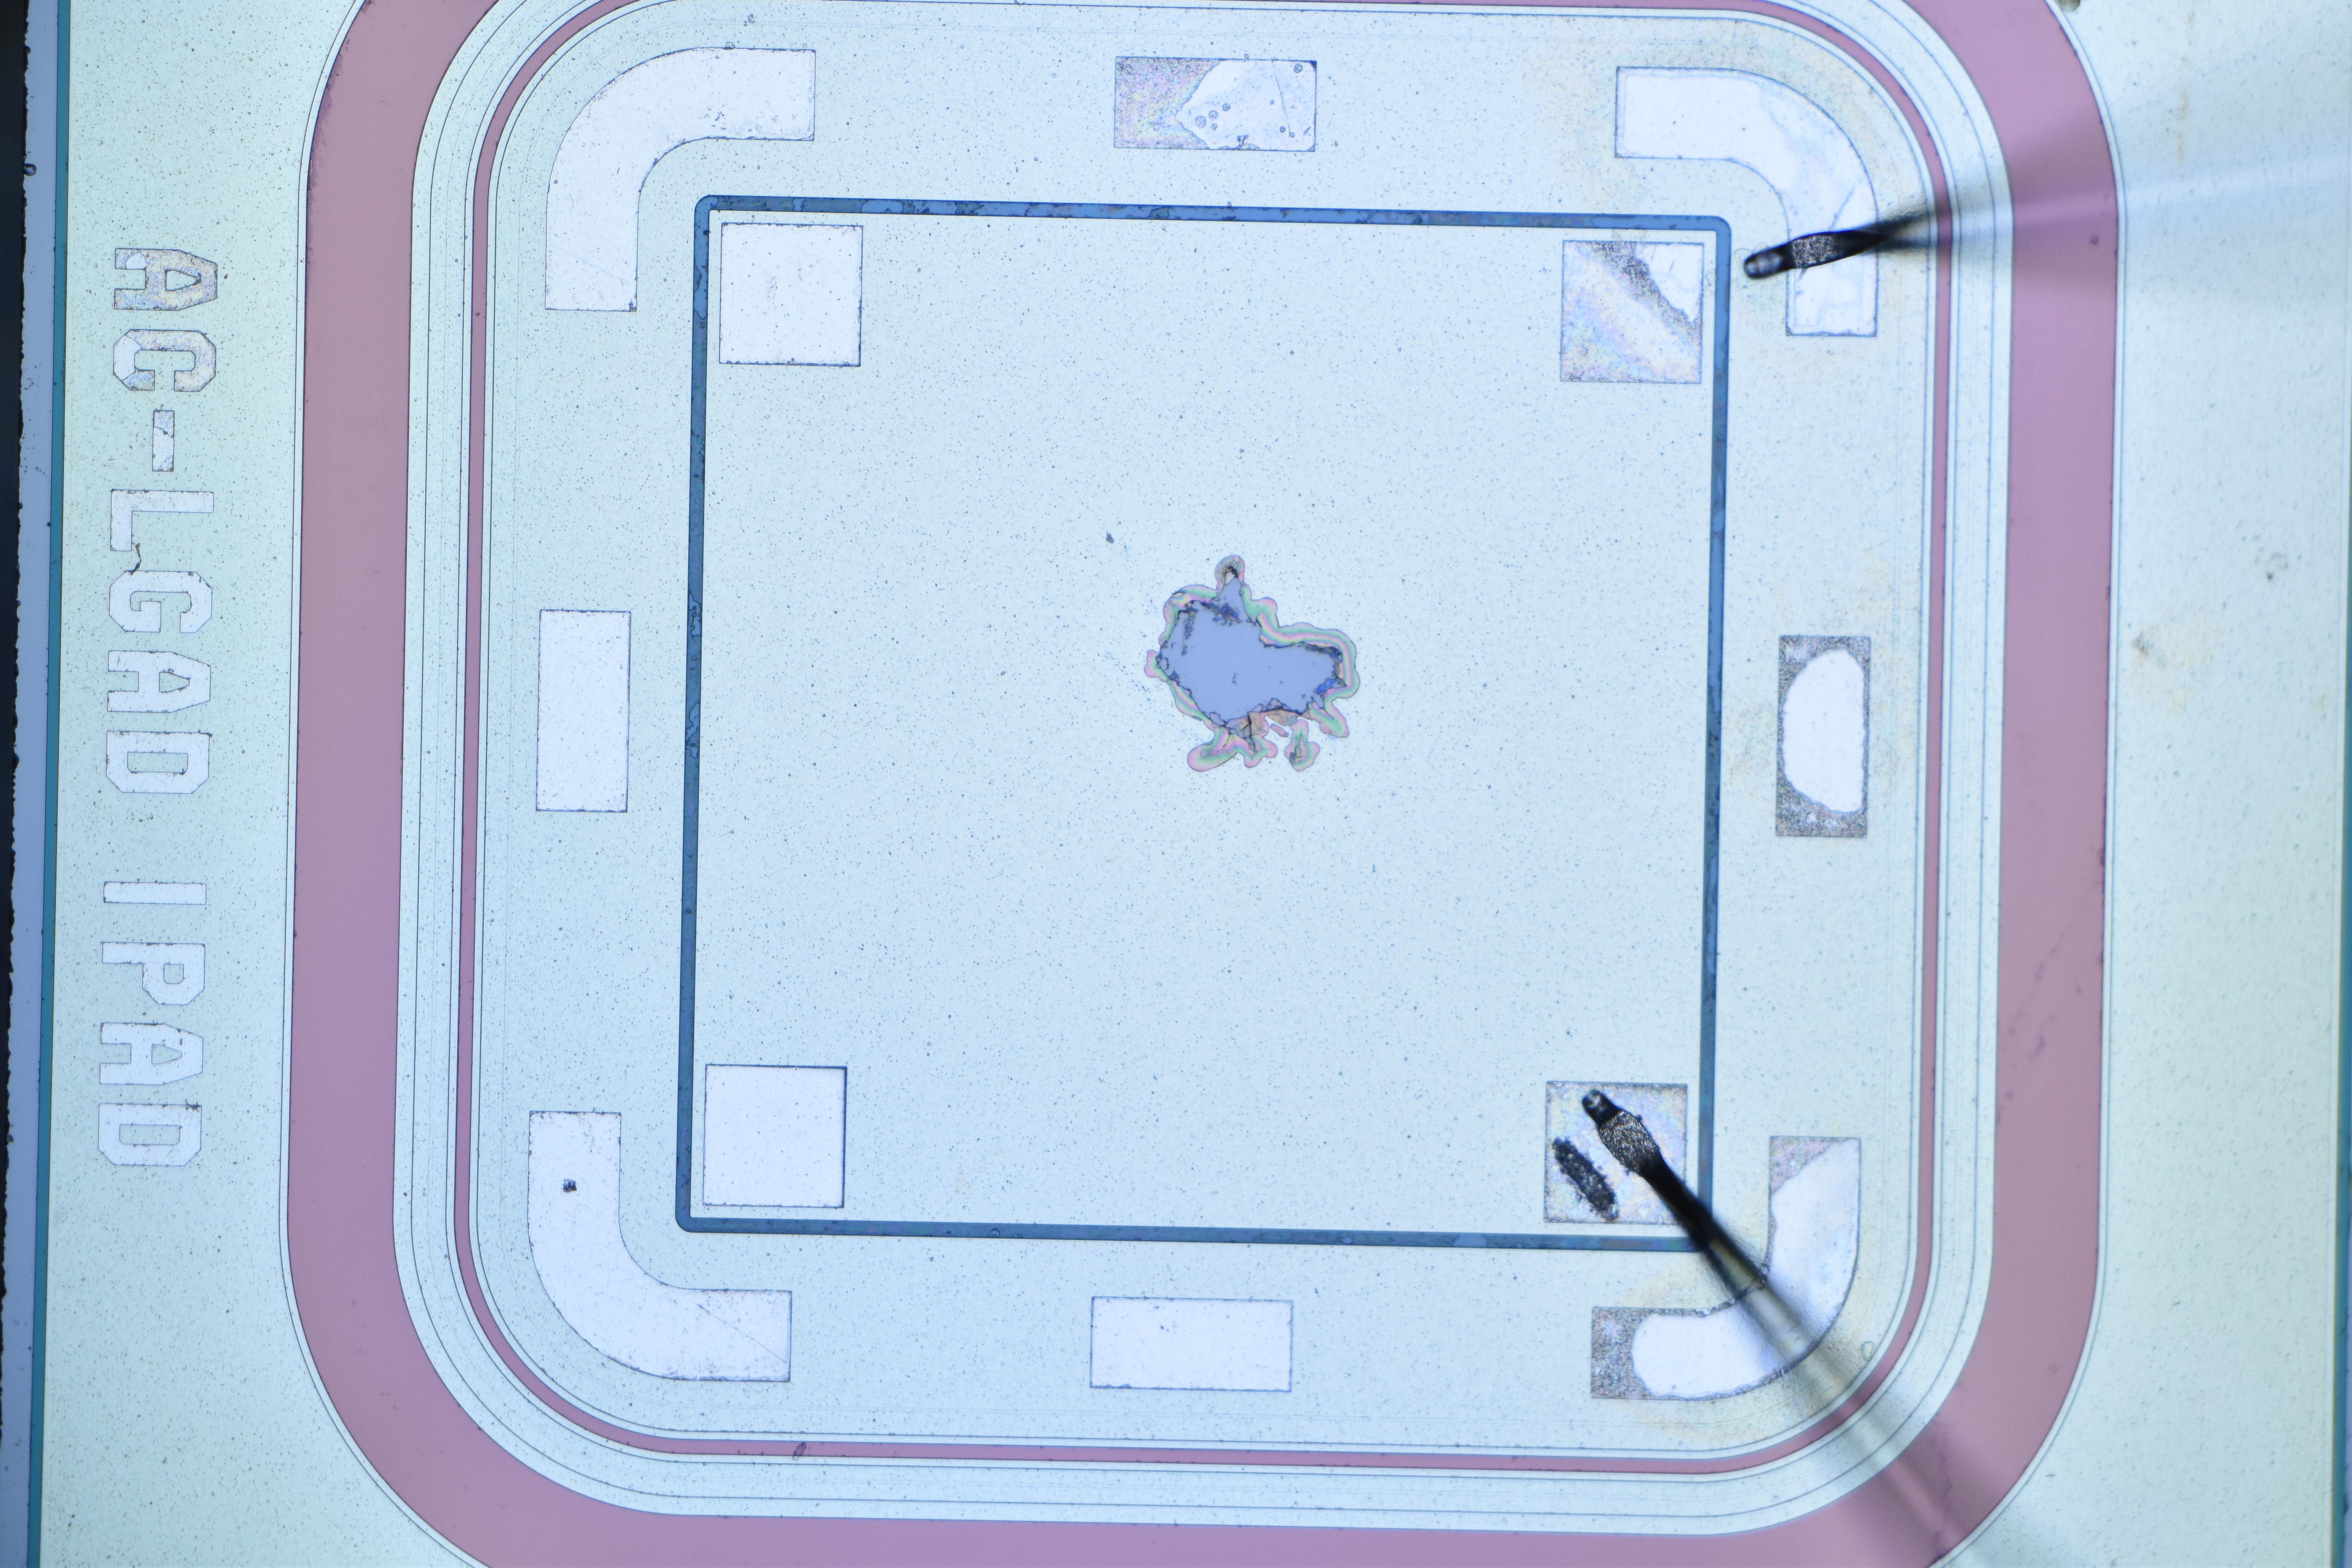
\includegraphics[width=5cm]{fig/ch4/PIN_front.jpeg}
        \subcaption{PIN}
        \label{fg:PIN_front}
    \end{minipage}
    \begin{minipage}[b]{0.5\linewidth}
        \centering
        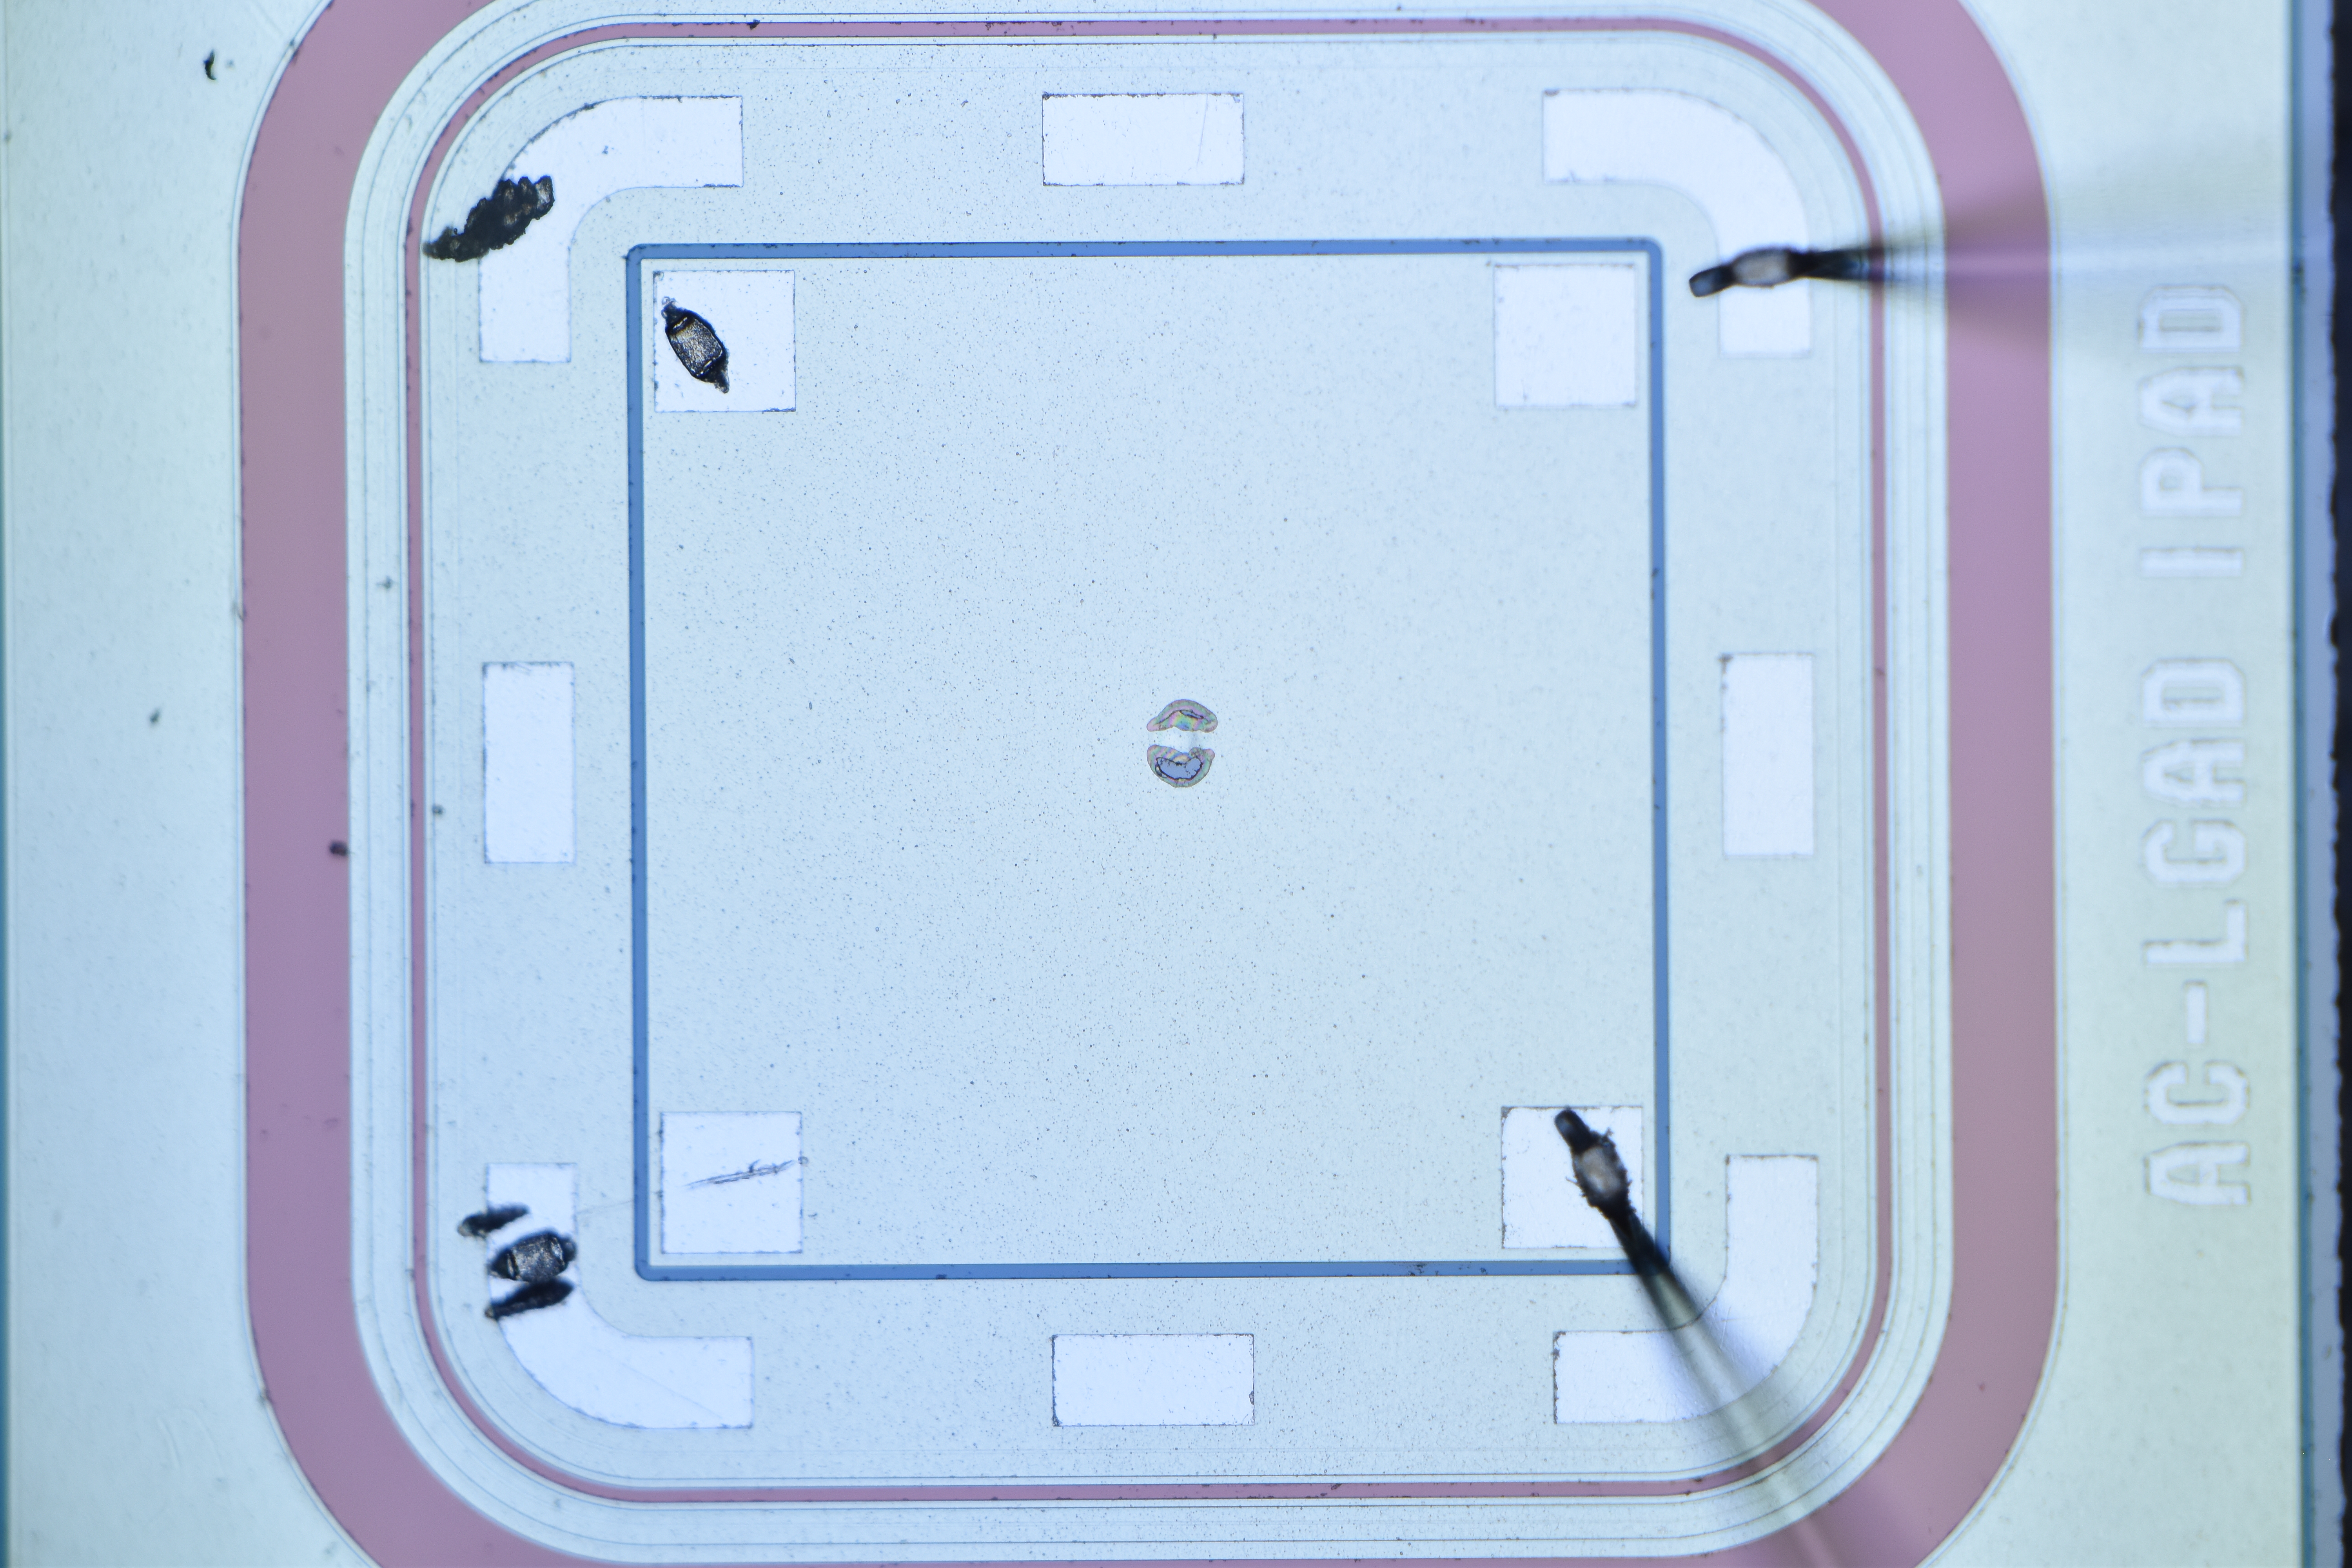
\includegraphics[width=5cm]{fig/ch4/APD_front.jpeg}
        \subcaption{APD}
        \label{fg:APD_front}
    \end{minipage}
    \caption[表面の剥離後の様子]{表面の剥離後の様子\\LGADとPINの中心の色が変わっている部分がアルミニウムを剥離して作成したレーザー窓。}
    \label{fg:front}
\end{figure}

\begin{figure}[h]
    \begin{minipage}[b]{0.5\linewidth}
        \centering
        \includegraphics[width=5cm]{fig/ch4/PIN_back.jpg}
        \subcaption{PIN}
        \label{fg:PIN_back}
    \end{minipage}
    \begin{minipage}[b]{0.5\linewidth}
        \centering
        \includegraphics[width=5cm]{fig/ch4/APD_back.jpg}
        \subcaption{APD}
        \label{fg:APD_back}
    \end{minipage}
    \caption[裏面の剥離後の様子]{裏面の剥離後の様子\\LGADとPINの中心の色が変わっている部分が裏面反射を防ぐためにアルミニウムを剥離した。}
    \label{fg:back}
\end{figure}

